{\LARGE Output:}

Plot the magnitude of X versus f: see {figure}[!h] for the ouput



 Is X nonzero at the proper frequency values? 

	Yes, the nonzero points were at 1000 and -1000 whihc corespond to $\Omega_0 =2\pi(1000)$ where 1000 is the the bandlimit occurs.


 Is the phase of X correct, assuming that the phase is equal to zero when X is nearly zero, I.E., nonzero only due to reound-off error.

	Yes, the phase of X is correct.

\begin{figure}[!htbp]
  \centering
    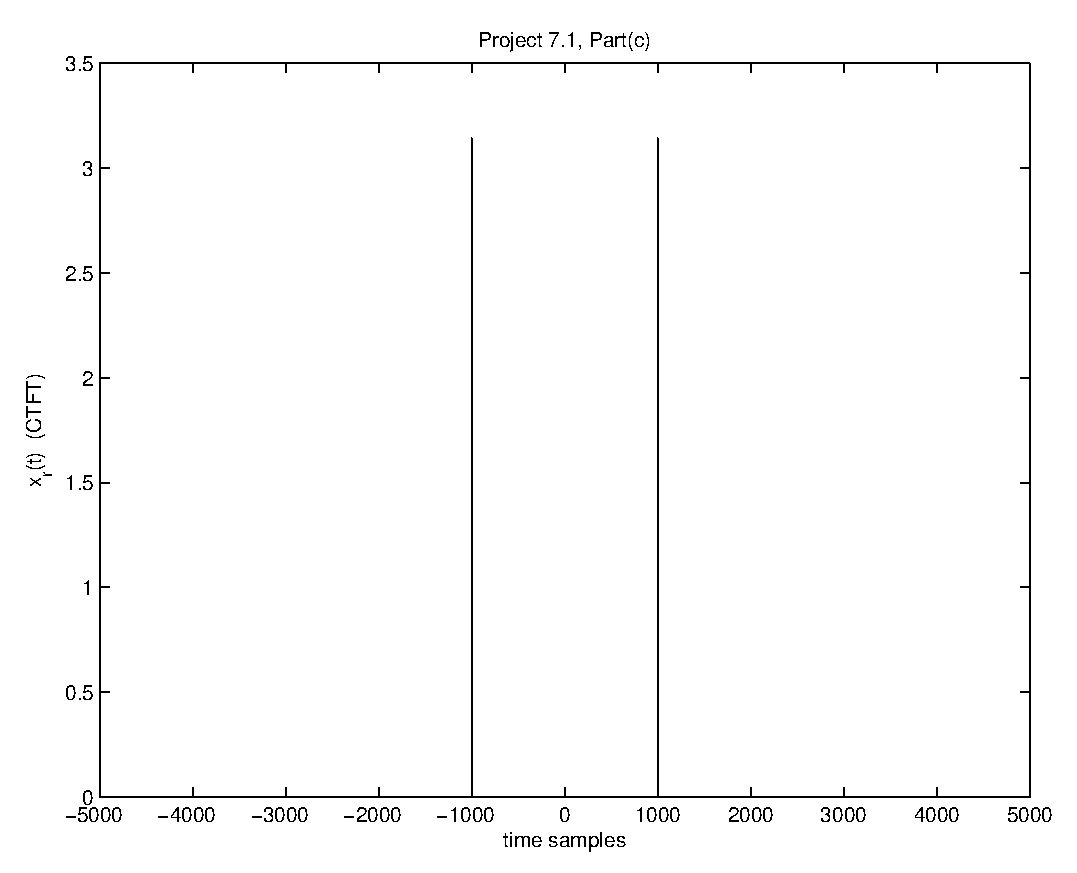
\includegraphics[width=0.7\textwidth]{Part1/Output/Figures/proj71PartC.eps}
  \caption{Output for 7.1 Part C}
\end{figure}

\pagebreak
